% R008 — Guide to Cultivating Complex Analysis (Bahasa Indonesia)
% Reader-facing translation unit: source/ca-v1.9/ca.tex lines 1414–1452.
% Source release: v1.9 (commit a4d25d9ba37a486a5a020219eb8bd4e6602fd14c).
% Translation provenance: OpenAI Codex gpt-5.6-sol, Ultra, acting on the user's request.
% Preserve source equations, notation, references, labels, figure paths, and caption text.

Perhatikan garis vertikal yang diberikan oleh $x=c$. Karena
\begin{equation*}
e^{z} =
e^{x+iy} =
e^x e^{iy}
\end{equation*}
dan $\sabs{e^{iy}} =1$, eksponensial memetakan garis vertikal $x=c$ ke
lingkaran berjari-jari $e^c$. Lihat \figureref{fig:expplotlines}.
Dengan demikian, eksponensial $w=e^z$ memetakan pita $a < x < b$ ke
anulus
\begin{equation*}
\bigl\{ w \in \C : e^a < \sabs{w} < e^b \bigr\} .
\end{equation*}

Di sisi lain, garis horizontal $y=c$
dipetakan ke sinar dari titik asal menuju tak hingga dengan $\theta = c$ dalam
koordinat polar. Lihat kembali \figureref{fig:expplotlines}.
Oleh karena itu, eksponensial memetakan pita $a < y < b$ ke
sektor
\begin{equation*}
\bigl\{ w \in \C : ``a < \arg w < b'' \bigr\} .
\end{equation*}
Alasan penggunaan tanda petik adalah bahwa pertidaksamaan tersebut tidak
bermakna tanpa penafsiran yang tepat. Maksudnya, setidaknya salah satu nilai
dari $\arg w$ berada di antara $a$ dan $b$.
Khususnya, eksponensial $e^z$ memetakan himpunan yang diberikan oleh
$2k\pi < \Im z \leq 2(k+1)\pi$ secara satu-ke-satu
(lihat \exerciseref{exercise:exponetoonestrip})
ke seluruh $\C \setminus \{ 0 \}$.

\begin{myfig}
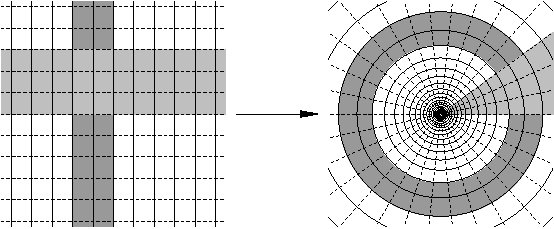
\includegraphics{figures/expplotlines}
\caption{Garis-garis horizontal dan vertikal, serta sebuah pita horizontal dan
sebuah pita vertikal, dipetakan oleh eksponensial. Perhatikan bahwa
setiap garis horizontal hanya dipetakan ke satu sinar dari titik
asal.\label{fig:expplotlines}}
\end{myfig}

%%%%%%%%%%%%%%%%%%%%%%%%%%%%%%%%%%%%%%%%%%%%%%%%%%%%%%%%%%%%%%%%%%%%%%%%%%%%%%
